\section{Diseño}

\subsection{Diseño de las clases de la Arquitectura}

Varios componentes interconectados conforman la arquitectura de implementación del sistema de generación de terreno procedural en Unity, los cuales trabajan juntos para lograr una generación y representación efectiva del terreno. Las clases y su papel en el proceso de creación del suelo las abordaremos con más detalle posteriormente. Los componentes que fueron elegidos durante la fase de análisis se han combinado para crear dos subsistemas para la generación de alturas y la generación del propio terreno.

\subsubsection{Generación de alturas}
Los Jobs, los cuales son unidades de trabajo paralelo que tienen como función la generación del terreno, la erosión y tareas intensivas en la CPU, entre otras.
\begin{itemize}
    
    \item \textbf{Noise}: se encarga de proporcionar métodos los cuales generan ruido Perlin, Simplex y Voronoi, estos son utilizados para crear mapas de altura del terreno. Entre sus características destacan:
			
    \begin{itemize}
        \item Generar ruido 3D y 2D utilizando los algoritmos citados anteriormente.
	\item Por medio de Unity Jobs y la biblioteca Burst, se puede generar ruido eficientemente.	
        \item Además, podemos configurar ciertos parámetros como son las octavas, la escala y la persistencia para así poder controlar la apariencia del terreno.
        
    \end{itemize}

    \item \textbf{ErosionJob}: Job que sirve para poder aplicar algoritmos de erosión al terreno que hemos generado.
    \begin{itemize}
        \item Para lograr resultados más realistas, este job permite que podamos trabajar conjuntamente a la configuración de erosión y el mapa de altura.
	\item Al calcular en cada punto del terreno la erosión térmica, nos permite suavizar las pendientes del terreno y mejorar así, la autenticidad de este.
        \item Facilidad para hacer simulaciones para el terreno con procesos de erosión realistas. 
    \end{itemize}

    \item \textbf{MapGeneratorJob}: 
    \begin{itemize}
        \item Job que nos permite generar el mapa de altura del terreno.
        \item Para poder crear el mapa de altura del terreno utilizamos algoritmos de ruido y la configuración de generación. 
        \item Para lograr un resultado eficiente computacionalmente, paralelizamos el procesamiento de cada vértice en diferentes hilos.
    \end{itemize}
    
\end{itemize}

\subsubsection{Generación y gestión del Terreno}
El generador de terreno gestiona la creación y visualización de chunks de terreno en el mundo del juego. Garantiza que solo se carguen chunks visibles y que se utilice el nivel de detalle (LOD) para optimizar el rendimiento.

\begin{itemize}
    \item \textbf{EndlessTerrain}:
    \begin{itemize}
    \item Responsable de gestionar la generación de nuevos chunks de terreno.
    \item Actualiza la posición del jugador y determina qué chunks se cargarán o descargarán. 
	\item Almacena y gestiona un diccionario de chunks mostrados en el mundo.	
	\item Utiliza niveles de detalle (LOD) para optimizar la definición del terreno según la distancia del jugador.
	
    \end{itemize}

    \item \textbf{TerrainChunk}:  
    \begin{itemize}
        \item Representa un pedazo de terreno individual.
       \item Actualiza y muestra una porción del terreno según su ubicación y nivel de detalle (LOD).  
	    \item Almacena la mesh del terreno y es responsable de su representación visual.
	    \item Administra solicitudes y recibe datos de mapas y cuadrículas con Jobs.
    \end{itemize}

    \item \textbf{MapGenerator}: 
    \begin{itemize}
        \item Crea mapas de elevación utilizando algoritmos de ruido y otros métodos para crear un terreno realista y detallado.
	    \item Controla parámetros como escala, octava y durabilidad para ajustar la apariencia del terreno.  
	    \item Utiliza Unity Jobs y la biblioteca Burst para generar ruido de manera efectiva.
    \end{itemize}

    \item \textbf{MeshGenerator}:
    \begin{itemize}
        \item Genera meshes de terreno con distintos niveles de detalle (LOD) para representación visual.
	    \item Permite transiciones suaves entre meshes LOD para evitar artefactos visuales.
	    \item Ejecuta consultas y obtiene mesh de terreno usando Job. 

    \end{itemize}

    \item \textbf{MeshDataGeneratorJob}: 
    \begin{itemize}
        \item Calcula la forma de la mesh, incluidos vértices, triángulos y coordenadas UV.
	\item Utiliza datos como mapas de elevación y parámetros de cuadrícula para crear cuadrículas de terreno. 
	\item Esta es una parte indispensable de la representación visual de las secciones del terreno.
    \end{itemize}

\end{itemize}

\subsubsection{Representación del Terreno}

Como se mencionó anteriormente, los propios bloques son responsables de gestionar la información y almacenar sus coordenadas de textura. Sin embargo, cuando se procesan los vértices para generar sus alturas, se creará un mapa paralelo, que es un mapa de colores, que luego se convierte en una textura que servirá para representar visualmente la Pieza.

\item \textbf{TextureGenerator}: Se encarga de crear texturas del terreno a partir de mapas de elevación y otros datos.
\begin{itemize}
    \item Crea texturas usando datos como mapas de altura y paletas de colores.
	\item Le permite personalizar asignaciones de texturas para diferentes elevaciones y características del terreno.
	\item Utiliza Unity Jobs para obtener texturas eficientemente.
\end{itemize}

\subsection{Diseño de la Arquitectura del Software}

\subsubsection{Diagrama de Clases}

 El siguiente diagrama de clases describe en detalle las relaciones entre los componentes del sistema.

\begin{figure}[H]
    \centering
    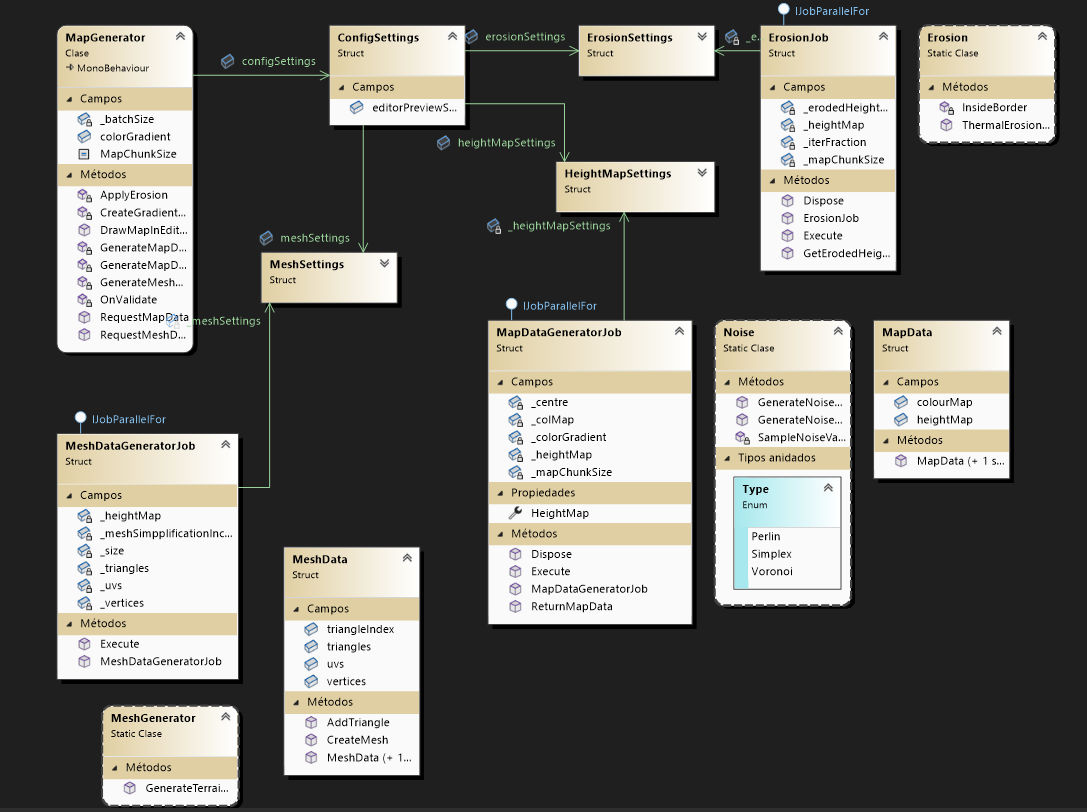
\includegraphics[width=1\textwidth]{img/diagrama de clases.png}
    \caption{Diagrama de Clases.}
\end{figure}
\newpage

\subsubsection{Diagramas de Secuencia}
Los diagramas de secuencia ilustran las interacciones entre los componentes clave del sistema.

\begin{figure}[H]
    \centering
    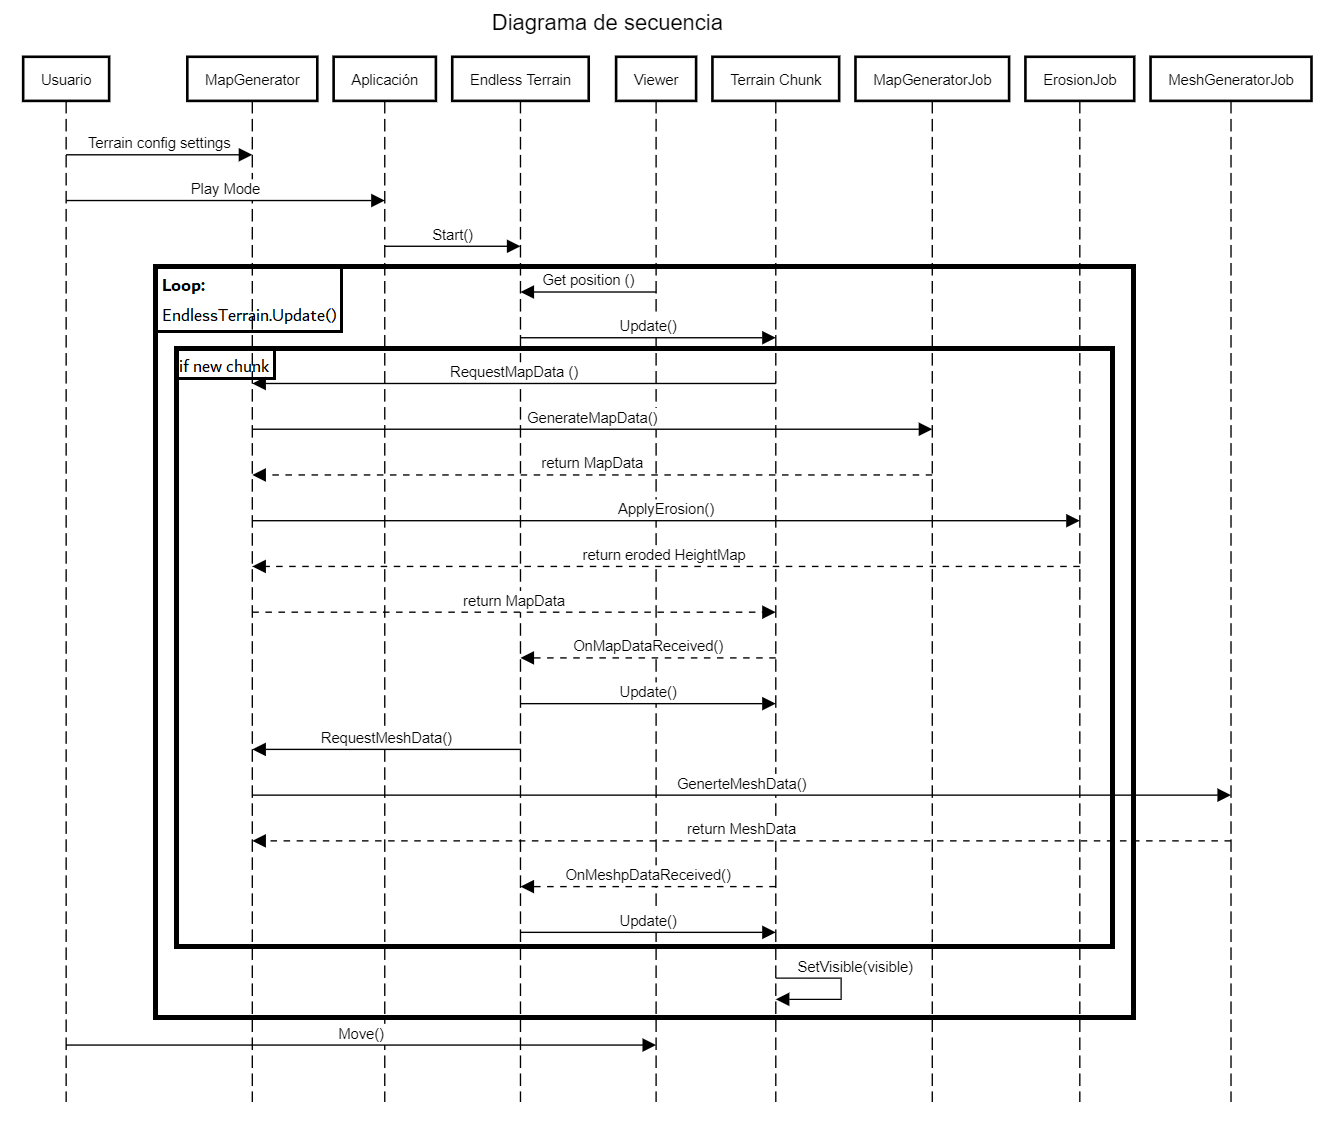
\includegraphics[width=1\textwidth]{img/Diagrama de secuencia.png}
    \caption{Diagrama de Secuencia.}
\end{figure}
\newpage

\subsection{Diseño Detallado}

\subsubsection{Diagramas de Flujo}
Los siguientes diagramas demuestran los flujos de trabajo y procesos entre los diferentes sistemas y componentes de la herramienta.

\begin{figure}[H]
    \centering
    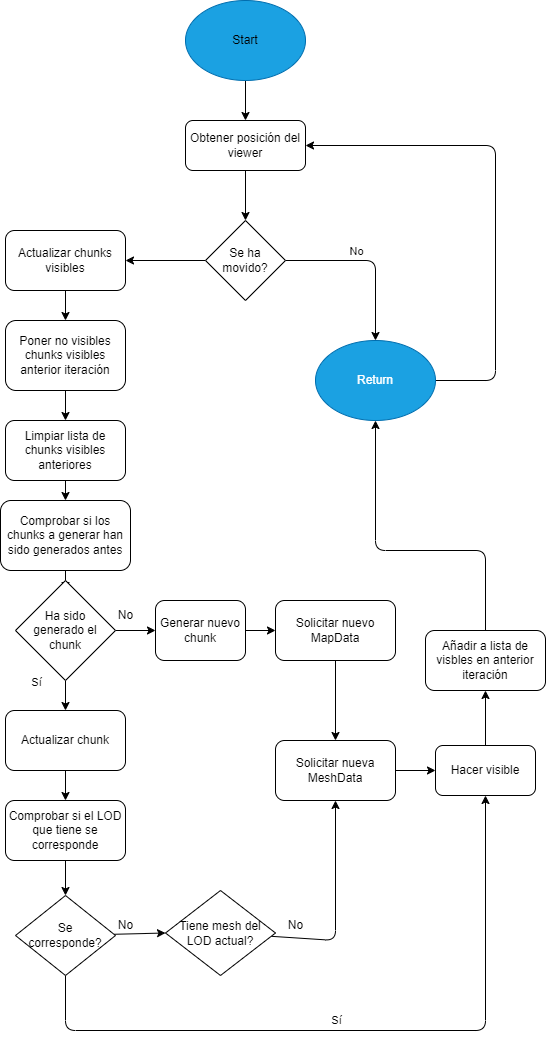
\includegraphics[width=0.65\textwidth]{img/FlowDiagramEndlessTerrain.png}
    \caption{Diagrama de Secuencia de Generación de Terreno desde el inicio de EndlessTerrain.}
\end{figure}
\newpage

\subsection{Desafíos y Decisiones de Diseño}

\subsubsection{Desafíos Técnicos}
Hubo algunos desafíos técnicos durante el diseño y desarrollo del proyecto. Los desafíos más notables incluyen:

\begin{itemize}
    \item \textbf{Optimización de Rendimiento:} Lograr un rendimiento óptimo en la generación de terreno procedural en tiempo real es uno de los desafíos técnicos clave. Se implementaron el sistema de tareas Unity y el compilador Burst para abordar este desafío.
    
    \item \textbf{Generación Realista:} Crear terrenos realistas y diversos implica implementar algoritmos de ruido Perlin, Simplex y Voronoi, así como configurar parámetros apropiados como escalas y octavas.
    
    \item \textbf{Erosión y Características Naturales:} La integración de algoritmos de erosión para simular características naturales como ríos y cañones plantea un desafío adicional. 
    
    \item \textbf{Continuidad del terreno:} La continuidad del terreno de nueva creación, sin darse cuenta de la transición entre las partes del terreno generado y su integración en el terreno existente, representa otro problema técnico a resolver.
    
    \item \textbf{Corrección de borde en erosión:} Cuando el proceso de erosión se hace teniendo en cuenta la elevación de cada terreno y equilibrándolas, se crean inconsistencias con el terreno. Resolver este problema presenta otro desafío.
    
    \item \textbf{Implementación de LOD:} Incluir LOD crea otro desafío porque si bien no es una función que se aplica en paralelo, es una función adicional que amplía las capacidades de la herramienta permitiendo que se pueda crear expansión del terreno a un costo menor que la generación cero completa. paralelismo.
    
    \item \textbf{Paralelización de la creación del mapa de altura:} La creación paralela de mapas de elevación ha dado lugar a cambios en la forma tradicional de crear mapas de elevación, lo que requiere ajustes.
     
    \item \textbf{Paralelización de la erosión del mapa de altura:} De manera similar a cómo paralelizar un mapa de elevación implica cambios en el método tradicional, la erosión implica una gran refactorización de la lógica para la que se diseñaron los algoritmos de erosión y a la que deben adaptarse para ser adecuados.
     
    \item \textbf{Paralelización de la creación del mapa de altura:} Finalmente, la configuración del array de vértices, uvs y triángulos de las meshes generadas también se debe realizar de forma procedimental por lo que al igual que en los dos casos anteriores es necesario estudiar cómo hacerlo de forma óptima. 
\end{itemize}

\subsubsection{Decisiones de Diseño}
Las decisiones de diseño juegan un papel clave en la arquitectura y funcionalidad de un proyecto. Algunas decisiones importantes incluyen:

\begin{itemize}
    \item \textbf{Uso del Unity Job System:} Se decidió utilizar el Unity Job System para paralelizar tareas y optimizar la generación de terreno, lo que mejora el rendimiento.
    
    \item \textbf{Selección de Algoritmos de Ruido:} La elección de implementar algoritmos de ruido Perlin y Simplex ayuda a crear terrenos realistas y diversos con una apariencia natural.
    
    \item \textbf{Erosión para Características Naturales:} La incorporación de algoritmos de erosión en el diseño permite la creación de características naturales como ríos y cañones, mejorando la apariencia general del terreno.
    
    \item \textbf{Uso de LOD:} Incorporar LOD al proyecto agrega una característica adicional, porque si bien no es una función que se aplica en paralelo, es una función adicional que amplía las capacidades de la herramienta permitiendo que se pueda crear expansión del terreno a un costo menor que la generación cero completa. paralelismo.
    
    \item \textbf{Elección de nave como explorador:} La elección de un barco como explorador del terreno se debió a las irregularidades del terreno en terrenos escarpados que podrían dificultar la exploración, además de que al sobrevolar se puede observar con mayor claridad el desempeño del sistema.
    
    \item \textbf{Configurabilidad:} Clases como "HeightMapSettings", "MeshSettings" y "ErosionSettings" están diseñadas para permitir una configuración flexible de diferentes configuraciones de terreno. Los usuarios pueden ajustar la escala de ruido, la resolución de la mesh y los efectos de erosión para adaptarlos a sus necesidades.
    
\end{itemize}

\subsubsection{Consideraciones de Rendimiento}
Durante el proceso de diseño, se tuvieron en cuenta varias consideraciones de rendimiento para garantizar un sistema eficiente: 
- \textbf{Optimización de la Malla:} La implementación de una lógica de generación de mesh eficiente reduce la cantidad de vértices y triángulos según el nivel de detalle, mejorando así el rendimiento de renderizado.

- \textbf{Burst Compiler:} El uso de la herramienta Burst Compiler compiló el código C\# en código nativo altamente optimizado, mejorando aún más el rendimiento de generación de terreno.

- \textbf{Paralelización:} Aprovechar el paralelismo a través del Sistema de Trabajo Unificado garantiza que la generación de terreno se ejecute de manera eficiente en sistemas con múltiples núcleos de CPU.

\subsection{Planificación de Desarrollo}

\subsubsection{Cronograma de Desarrollo}

El desarrollo de este proyecto se ha planificado en varias fases, con hitos de finalización y fechas importantes:

 \textbf{Análisis preeliminar:} En esta etapa, se realizó una investigación previa sobre los algoritmos de generación del terreno, se plantaron los primeros requiisitos y se diseñó la planificación del desarrollo del proyecto. Esta fase finaliza con el hito de la aprobacion del análisis preeliminar

 \textbf{Análisis:} En esta fase se termiann de determinar los requisitos más en profundidad, se hace un estudio de los componentes que deben estructurar la arquitectura y se hace un análisis de los procesos que deben intervenir. Esta fase finalzia con la aprobación del análisis.

 \textbf{Diseño:} Se diseña la arquitectura del sistema, los procesos, compoentnes y las parametors que darána la configurabilidad a la herramienta. Se finaliza esta etapa tras el hito de la aprobación del diseño

 \textbf{Implementación:} Realización de los sistemas persé. Se desarrollan todos los compoenentes necesarios para el funcionamiento de la herramienta. Finaliza tras la optimización. 

 \textbf{Pruebas:}En esta fase se pone a prueba la implementación y se mejoran las fallas encontradas. Se finalzia con la comprobación y aprobación de los resultados.
 
 \textbf{Finalización de la documentación:}En esta fase se hace una memoria y se crea un video demo donde se muestren las caracterísitcas y funcionalidades de la herramienta.


 Se puede ver el cronograma del desarrollo en el apéndice: 

\subsection{Conclusión}

En resumen, esta sección proporciona una descripción general del diseño de nuestro sistema, destacando decisiones clave, consideraciones de rendimiento y planificación de desarrollo. Durante el proyecto, continuaremos refinando y mejorando esta arquitectura para lograr nuestros objetivos. En las siguientes secciones, nos centraremos en la implementación y prueba del sistema.
